\chapter{Hardware}
%http://samurai1967.dyndns.org/avr-net-io.html
%http://www.fhemwiki.de/wiki/AVR-NET-IO
%http://www.mikrocontroller.net/articles/AVR_Net-IO_Bausatz_von_Pollin
\section{AVR Net-IO-Board}
\begin{figure}[h]
\centering
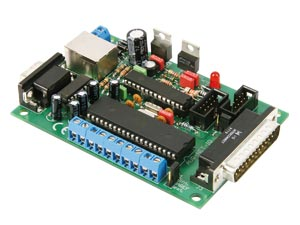
\includegraphics[width=10cm]{content/pictures/avr-net-io.jpg}
\caption{AVR-NET-IO - Pollin GmbH}
%http://www.pollin.de/shop/dt/MTQ5OTgxOTk-/Bausaetze_Module/Bausaetze/Bausatz_AVR_NET_IO.html
\label{fig:B3}
\end{figure}

\subsection{Technische Daten}
\begin{itemize}
  \item Betriebsspannung 9V
  \item Stromaufnahme ca. 190 mA
  \item 8 Digitale Ausgänge, 4 Digitale Eingänge
  \item 4 Analoge Eingänge
  \item ATmega32 Mikrocontroller
  \item integrierte ISP-Schnittstelle
\end{itemize}

\section{Mikrocontroller}
\subsection{ATmega32}

\subsection{ATmega644P}

\subsection{ATmega1284P}

\subsection{ENC28J60}

\section{Fuse Bits}
\label{chap:Fuse}

Die Fuse-Bits sind die Grundlegenden Einstellungen, mit denen ein
Mikrocontroller arbeitet. Sie müssen geändert werden, wenn ein anderer Taktgeber
gewünscht ist oder Schnittstellen de- oder aktiviert werden sollen.

\begin{table} [H]
\begin{tabular}{|l|l|l|} \hline
Fuse Name & Bedeutung & Bytes\\ \hline
BODLEVEL & Brown-out Detector trigger level & E-Fuse 0\&1\\ \hline
OCDEN & Aktiviert On-Chip Debuging & H-Fuse 7\\ \hline
JTAGEN & Aktiviert das \ac{JTAG} Interface & H-Fuse 6\\ \hline
SPIEN & Aktiviert das \ac{ISP} Interface & H-Fuse 5\\ \hline
WDTON & \ac{WDT} immer an & H-Fuse 4\\ \hline
EESAVE & Schützt den \acs{EEPROM} wärend des Lösch-Zyklus & H-Fuse 3\\ \hline
BOOTSZ & Boot Flash Sektor Größe & H-Fuse 1\&2\\ \hline
BOOTRST & Boot Reset Vektor & H-Fuse 0\\ \hline
CKDIV8 & Teilt den Takt der Uhr intern durch 8 & L-Fuse 8\\ \hline
CKOUT & Ausgabe des Takts der Uhr auf Port B1 & L-Fuse 7\\ \hline
SUT\_CKSEL & Wahl der Takt-Quelle & L-Fuse 0-6\\ \hline
\end{tabular}
\caption{Die Bedeutung der einzelnen Fuse-Bits (ATMega-664P)}
\label{fuses}
\end{table}